\documentclass{article}

\usepackage[margin=1.5in]{geometry}
\usepackage{graphicx}
\usepackage[hidelinks]{hyperref}
\usepackage{pdfpages}
\usepackage{enumitem}
\usepackage{tabularx}
\usepackage{float}

\newcommand{\IMAGEPATH}{../Images/}

\newcolumntype{Y}{>{\centering\arraybackslash}X}

%opening
\title{UAV Outback Challenge 2016\\ \large Deliverable \#2\\}

\author{
	\textbf{Melbourne Autonomous Systems}\\
	Matt De Bono,
	Alex Daraio,
	Bede Wolfenden,\\
	Frankie Lanciana,
	Sophie Bainbridge,
	Nathan Murfey}

\begin{document}

\maketitle

\textbf{Picture of Dragonfly here.}

\newpage

\tableofcontents

\newpage

\textbf{All information is taken from pages 24 and on from the UAV Challenge Rules specification. Deliverable \#2 is to be a maximum of 23 pages.}\\

\textbf{In addition to this report, teams must submit a flight demonstration video. The video must demonstrate autonomous take-off and landing, and pre-flight set up and checks.}\\

Team submissions are assessed according to Figure \ref{fig:D2Scoring}.

\begin{figure}[h]
	\centering
	\includegraphics[width=\linewidth]{\IMAGEPATH D2Scoring}
	\caption{Scoring for Deliverable \# 2}
	\label{fig:D2Scoring}
\end{figure}

\section{Tasks for Deliverable \#2}
Create a video that shows:
\begin{enumerate}
	\item Pre-flight set up and checks
	\item Autonomous takeoff and landing of Retrieval Aircraft
\end{enumerate}

The report must demonstrate:
\begin{enumerate}
	\item Aircraft must automatically engage their \textit{Flight Termination System} if they breach the Geofence
\end{enumerate}

To be added to the UAV (if possible):
\begin{enumerate}
	\item Backup power system
	\item External emergency stop button
	\item External arming switch and state indicator (LED)
\end{enumerate}

From the ``Go'' email:
\begin{enumerate}
	\item If you have a VTOL system, you need to ensure that you address the case of GPS failure during all modes of flight, especially hovering. How will you hover if you do not have GPS?
	\item Consider the potential for multiple failures and how certain combinations of failures may require flight termination.
	\item Please ensure that there is sufficient design information about your Flight Termination System in your D2 document so that the committee can confirm that it complies with the rules.
	\item You MUST ensure that any radio systems that you use are LEGAL in Australia (you MUST check this yourselves). You are not required to report the full details regarding your RF transmitters until D3, but you will not be given a Go decision at D3 if you are using illegal frequencies or illegal radiated power levels.
	\item Do not assume that aircraft will have reliable 3G or 4G mobile phone coverage during the mission. The mission may take place in an area of no, or poor mobile phone coverage.
\end{enumerate}

\section{Sections yet to be Completed}
\begin{itemize}
	\item Introduction and Design Approach
	\item Landing site analysis and strategy
	\item Test Results and Discussion
	\item System Design
	\item Risk Assessment
	\item Risk Management
	\item \textit{After other sections -} Conclusions
	\item \textit{After Conclusions -} Executive Summary
	\item \textit{After completing report -} Compliance Statement
\end{itemize}

\newpage

\section{Statement of Originality and Accuracy}
We declare that this report is entirely the work of the team members listed below, and has not previously been submitted by us, or others for this challenge or any other similar event.\\

We have acknowledged external material with appropriate references, quotes or notes to indicate its source.\\

We declare that this report is an accurate record of activities carried out by us in preparing for this specific challenge. The events, data and other material contained within this report actually occurred and have been fully detailed.\\

Participating team members:
\begin{itemize}
	\item Matt De Bono
	\item Alex Daraio
	\item Sophie Bainbridge
	\item Bede Wolfenden
	\item Frankie Lanciana
	\item Nathan Murfey
\end{itemize}

\newpage

% Append the Compliance Statement to the document
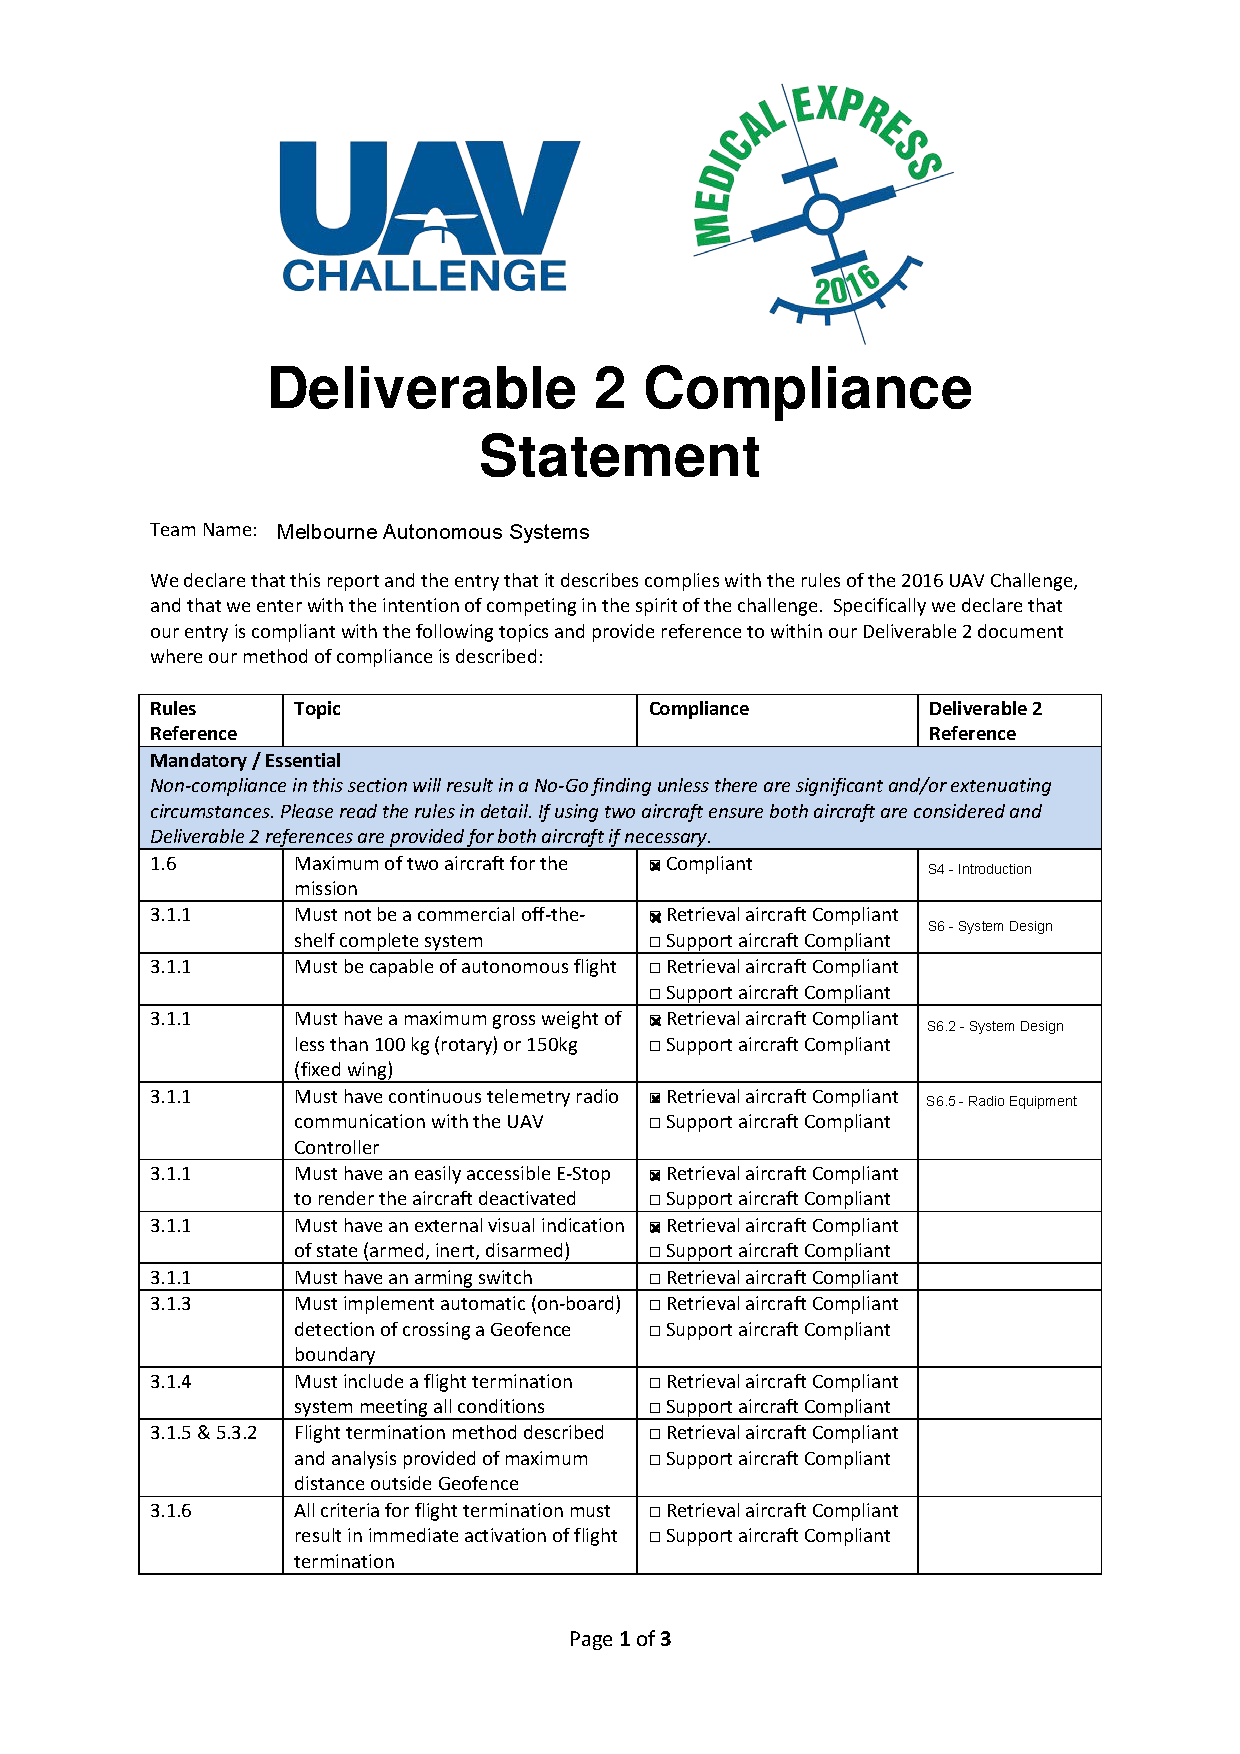
\includepdf[pages=-]{compliance.pdf}

\newpage
\section{Executive Summary (1 page)}
Summarise the document below; most likely a summary of our design, and our approach to maximise safety and compliance.\\

\textbf{This will be the final task of the report.}

\newpage
\section{Introduction and Design Approach (1 page)}
This Deliverable discusses the development and capabilities of Melbourne Autonomous Systems' entry to the 2016 UAV Challenge.\\

Discuss PixHawk as flight controller, and Pi as brains and compute center.\\

Overview of hybrid approach, and transition system.\\

List sensors included on aircraft.\\

We will use a single aircraft.\\

Not a commercial off-the-shelf solution.\\

State the aircraft's total weight.\\

\newpage
\section{Landing site analysis strategy (1 page)}
\subsection{Locating Joe}
Upon successfully reaching the end of the transit corridor, the aircraft will reduce altitude to 150 ft and slow to a controllable fixed wing flight, while maintaining speed above stall speed. Inside the Remote Landing Site a spiral search pattern will be implemented. It is assumed that the Remote Landing Site is centered at Joe's location and his location has an accuracy of plus or minus 100 meters.\\

With this in mind, the drone will navigate itself to the border of the reported area (lining up with a circle whose radius is 100 meters from Joe’s reported location). Once the aircraft has lined up with the circle it will start processing the images received from the camera mounted in the nose of the aircraft. It will continue along this path, every revolution bringing it slightly closer to the center until the 200 meter diameter circle has been searched in it’s entirety.\\

An on board companion computer (Raspberry Pi™) will use open source visual computation software OpenCV to process the incoming images in an attempt to identify any object on the ground that might match Joe's description. The visual processing will include (blue) color masking and recognition, edge detection and possibly human/facial recognition, as well as a machine learning layer. Objects will be given scores based on the likelihood that they are Joe, and when an object scores above a threshold the aircraft will attempt to further identify the object. At this point the approximate position of the object and the current position in the holding pattern will be recorded.\\

The aircraft will then move from fixed wing mode to hover-mode.Once in hover mode the aircraft will return to the recorded position and reacquire the object. Using the mounting angle of the camera and repeated altitude measurements (checked with GPS and barometric sensors) the Raspberry Pi will calculate the distance from the aircraft to the object. Using these more precise conditions the drone will move closer to the object and further attempt to identify it as Joe. Once the aircraft is satisfied that Joe has been found it will begin maneuvers (see below) in an attempt to perform a safe landing.\\

Should the aircraft decide that the item was a false positive, it will regain altitude, discard the object in memory, re-engage fixed wing flight and return to the stored location in the holding pattern to continue the search, repeating the above process with any object scoring a higher identification score than the threshold. 

\subsection{Finding a landing point}
Having calculated Joe's position, the area around Joe is recorded and an approximate landing site computed using OpenCV to find a  ``debris-free'' site, more than 30 meters from Joe, but less than 50 meters (for maximum points). The aircraft will fly in reverse until the camera is upon the proposed landing area and perform a more thorough search of the area with OpenCV in an attempt to identify any likelihood of failure upon landing due to collision. If any object is detected, the aircraft will strafe right while still keeping Joe centered and measure the next site. Then the aircraft will slowly move forward and land in the appropriate site, and then disarm.

\newpage
\section{System Design (4 pages)}
\subsection{System Diagrams}
\begin{figure}[H]	
	\begin{subfigure}{0.32\textwidth}
		\centerline{\includegraphics[width=270pt]{\IMAGEPATH sw-arch}}
		\caption{Software Architecture}
		\label{fig:sw-arch}
	\end{subfigure} %
	\begin{subfigure}{.93\textwidth}
		\centerline{\includegraphics[width=315pt]{\IMAGEPATH hw-arch}}
		\caption{Hardware Architecture}
		\label{fig:hw-arch}
	\end{subfigure}
	\caption{Architecture Diagrams}
	\label{fig:arch}
\end{figure}

\subsection{Aeronautical Requirements}
\begin{itemize}
	\item \textbf{Lift} - With our selection of motors and batteries, our UAV is capable of 6.5kg of lift, more than enough to lift the 4kg airframe, as well as accept the sample from Joe.
	\item \textbf{Stall} - As mentioned in Section \ref{sec:intro}, our UAV is built on the Skywalker X8 airframe. The stall speed of our aircraft is estimated to be 25.3 knots, according to empirical data on the Skywalker X8.
	\item \textbf{Speed} - The X8 has been demonstrated by many users to achieve airspeeds in excess of 75.5 knots using similar battery and motor selections.
	\item \textbf{Endurance} - Battery tests have shown that 4 vertical take-off and landing maneuvers, reaching an altitude of 20ft, lasting 1-2 minutes each, consumed only a small portion of total power capacity. Taking this into consideration, we have more than enough battery to achieve the remainder of the mission in fixed-wing flight.
	\item \textbf{Geofence Avoidance} - In order to maximise our chances of completing the challenge, the aircraft's position and orientation will be measured by the PixHawk's inbuilt IMU and accelerometer, as well as a 3DR GPS/compass module. In addition to this, altitude will also be measured by an altimeter, and a LiDARLite and ultrasonic sensor mounted beneath the airframe. All AMSL altitudes will be measured in pressure altitudes.
\end{itemize}

Prior to transitioning from hover to fixed-wing mode, the aircraft will align itself with wind, and the front rotors will be tilted at 30-45$^o$ to provide horizontal and vertical thrust. The aircraft will accelerate to above stall speed, at which the front rotors are fully rotated, completing the transition. To transition back to hover, the reverse operation is performed.\\

As the aircraft is not yet fully complete, the requirements above are estimation/calculations only. Full testing and validation will be performed prior to Deliverable 3, once the aircraft has progressed in development. At this point proper range and endurance tests to will be conducted get a better estimation of cruise speeds, take off, landing and sample pick up times, as well as maximum flight time.

\subsection{Flight Termination System}
\subsubsection{Design}
This aircraft’s flight termination system uses the on-board PixHawk controller and is built off existing APM:Plane firmware, with the focus of ensuring safe operation within a defined region of airspace, rather than prioritizing keeping the aircraft itself intact. Though our aircraft is a hybrid, it will respond as a fixed-wing device, disarming motors and setting  if the flight termination system is activated (i.e. motors will be disarmed and control surfaces will be set to the required positions). These control surface settings will cause the UAV to enter a spin towards the ground, thereby minimising the distance travelled beyond a Geofence boundary if a breach occurs.\\

The rationale behind this decision is that even in copter flight modes, the UAV still has wings that may catch the wind and carry it further beyond a breached geofence boundary, so to minimise distance travelled outside the geofence in all cases the following control surface settings will be imposed on the aircraft:
\begin{itemize}
	\item Throttle closed
	\item Full down on right aileron
	\item Full up on left aileron
	\item Rudder, elevator and flap controls are not applicable for our aircraft
\end{itemize}

As per the requirements of the UAV Challenge, this flight termination system can be triggered in manual or in automatic flight modes, and once activated cannot be overridden. The flight termination system is activated by:
\begin{enumerate}
	\item Geofence breach - The aircraft will automatically engage its flight termination system in the event of a Geofence breach (horizontal or vertical). This condition is checked on a 1Hz loop.
	\item Failure (or ‘lock-up’) of Geofence detection systems - If all sensors responsible for Geofence detection (IMU, accelerometer GPS, altimeter, LiDAR and ultrasonic), the aircraft can no longer measure its position, and should immediately engage flight termination.
	\item Manual activation - At any time during the mission, the flight termination system can be activated manually from the ground control station, overriding all actuators.
	\item Failure (or ‘lock-up’) of autopilot - Normal operation of the autopilot system is checked via ‘heartbeat’ signals provided at a frequency of 10Hz to the flight termination system. If these checks fail for a sustained period of 1 second, the flight termination system will be activated `immediately.
	\item Loss of both GPS and telemetry to GCS - A ‘heartbeat’ signal is also continually sent to the Ground Control Station via the telemetry link, to achieve the required 1Hz data update format. Failure to maintain this link during GPS failure will trigger the flight termination system.
\end{enumerate}

\subsubsection{State Machine}
Refer to Figure \ref{fig:termination-diagram}.
\begin{figure}
	\centering
	\includegraphics[width=1.1\linewidth]{\IMAGEPATH termination-diagram}
	\caption{State Machine for Flight Termination System}
	\label{fig:termination-diagram}
\end{figure}

\subsubsection{Analysis}
Calculating the worst case scenario for activation of the flight termination system following a Geofence breach, we assume the control surface settings will cause the plane to enter a near-vertical dive. However, for simplicity of analysis and to take a conservative approach, in calculating the worst-case the plane is treated as a simple falling mass (in reality, trajectory of its crash will be steeper and the distance travelled beyond the geofence will be shorter). Since this is a worst-case calculation, it was assumed that in this scenario the UAV is flying directly at a geofence boundary, at maximum speed and maximum allowable altitude.
\begin{itemize}
	\item Max speed = 75.5 knots = 38.5833m/s
	\item Max altitude = 1500ft = 457.2m
	\item Time to descend (as point mass under gravity) = 9.65s
	\item Horizontal distance travelled = 372m
\end{itemize}

\subsection{Geofence System}
The Geofence system implemented, as part of the firmware on our UAV, will be based on the system included in APM:Plane; that is, it will consist of a irregular polygon boundary made up of no more than 18 points, and will encompass the Base, the Landing Site, and the Transit Corridor.\\

Upon arming, a square Geofence will be sent to the PixHawk encompassing the Base. A soft Geofence will also be implemented as a circle of 800m diameter, allowing the UAV to attempt to recover when approaching the Geofence.\\

Once cruising altitude is reached, Geofence is modified to include the transit corridor and landing site. Given that teams are provided with the mission details at the commencement of the event, the soft Geofence for this section will be manually created by the team, such that the UAV can avoid flight termination in the Transit Corridor.\\

Finally, once reaching the landing site a square Geofence is again sent to the UAV, with the soft Geofence again being an 800m circle, centered on Joe's GPS location. When returning to Base, the Transit Corridor and Base Geofences are applied in the same manner.

\subsection{Radio Equipment}
In order to perform low-bandwidth digital telemetry between the drone and ground station over distances up to 12.5km we have chosen to use an RFD900 long range telemetry kit. In accordance with the ACMA LIPD-2015 ISM Class License this kit allows us to operate in a spectrum that does not require any specialised qualifications or license fees. The transmitter itself is compliant with AS 4268:2008, and is therefore suitable for use under the class license.\\

This kit operates between 902 and 928MHz, however we will use the 915-928MHz band in order to meet class license specifications.  Additionally the kit will be run at 1 Watt EIRP with at least 20 frequency hopping channels. Operating under these conditions falls under LIPD-2015 item 54 – Frequency Hopping Spread Spectrum transmitters.\\

If we find the low bandwidth telemetry link to be unreliable, a second transmitter will be added to provide communication redundancy. In accordance with the class license this will operate between 5725 and 5850MHz at 4 Watt EIRP, with at least 75 frequency hopping channels (LIPD-2015 item 57).

\newpage
\section{Risk Assessment (3 pages)}
\label{sec:risk-assessment}
The following tables identify various risks and hazards associated with the use of our aircraft, following a standard University of Melbourne Risk Assessment template, shown in Figure \ref{fig:risk-matrix}.\\

Each row of the risk assessment tables contains the following information: the potential hazard, the likelihood of that hazard occurring during the mission, a ``rating'' of the consequence of that hazard, and an assessment of the overall risk for that hazard. Management and mitigation of these risks will be discussed in Section \ref{sec:risk-management}.

\begin{figure}[H]
	
	\begin{subfigure}{\linewidth}
		\centerline{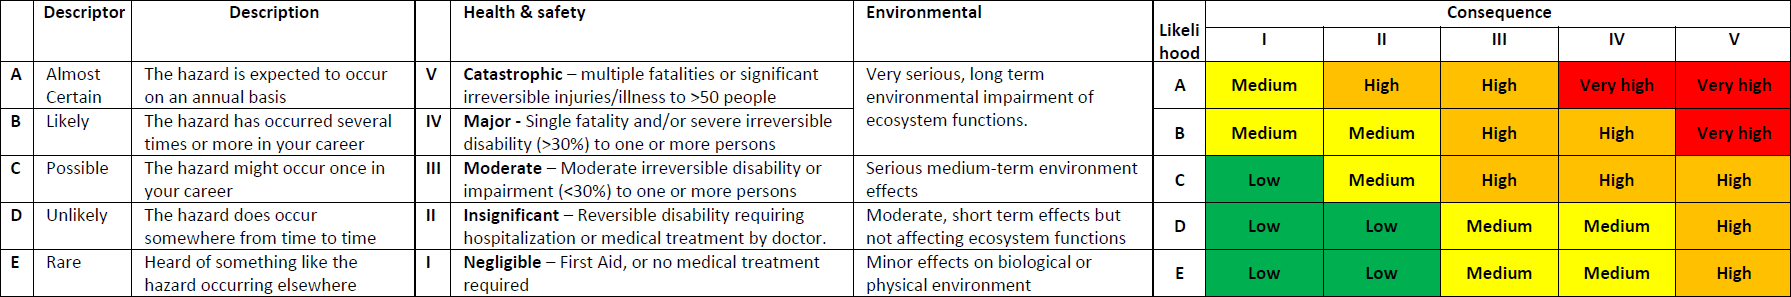
\includegraphics[width=550pt]{../Images/risk-matrix}}
	\end{subfigure}\\[2ex]
	
	\begin{subfigure}{\linewidth}
		\centerline{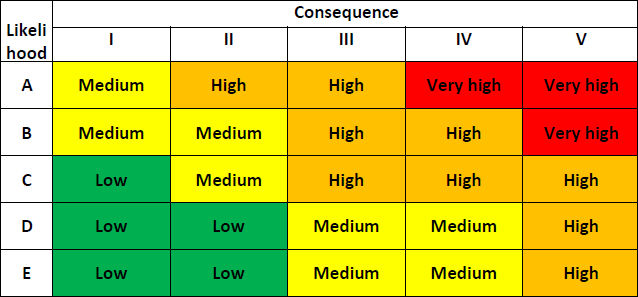
\includegraphics[width=300pt]{../Images/risk-matrix-2}}
	\end{subfigure}
	
	\caption{Risk Management Matrix}
	\label{fig:risk-matrix}
\end{figure}

\begin{table}[!h]
	\label{tab:risks-electrical}
	\centering
	\begin{tabularx}{\textwidth}{|Y|c|c|c|}
		\hline
		\textbf{Risk} & \textbf{Likelihood} & \textbf{Consequence} & \textbf{Risk Rating}\\
		\hline
		Electrocution & Possible & Insignificant & Medium\\
		\hline
		Impact to batteries & Possible & Insignificant & Medium\\
		\hline
		Loss of motor power & Possible & Insignificant & Medium\\
		\hline
	\end{tabularx} 
	\caption{Risk Assessment - Electrical Hazards}
\end{table}

\begin{table}[!h]
	\label{tab:risks-preflight}
	\centering
	\begin{tabularx}{\textwidth}{|Y|c|c|c|}
		\hline
		\textbf{Risk} & \textbf{Likelihood} & \textbf{Consequence} & \textbf{Risk Rating}\\
		\hline
		 & & & \\
		\hline
	\end{tabularx} 
	\caption{Risk Assessment - Pre-flight Hazards}
\end{table}

\begin{table}[!h]
	\label{tab:risks-autonomy}
	\centering
	\begin{tabularx}{\textwidth}{|Y|c|c|c|}
		\hline
		\textbf{Risk} & \textbf{Likelihood} & \textbf{Consequence} & \textbf{Risk Rating}\\
		\hline
		& & & \\
		\hline
	\end{tabularx} 
	\caption{Risk Assessment - Autonomous Takeoff and Landing}
\end{table}

\begin{table}[!h]
	\label{tab:risks-inflight}
	\centering
	\begin{tabularx}{\textwidth}{|Y|c|c|c|}
		\hline
		\textbf{Risk} & \textbf{Likelihood} & \textbf{Consequence} & \textbf{Risk Rating}\\
		\hline
		Loss of aircraft control & Possible & Insignificant & Medium \\
		(Autopilot failure or lock-up) & & & \\
		\hline
		Loss of aircraft control  & Likely & Insignificant & Medium \\
		(Propeller or power loss) & & & \\
		\hline
		Loss of GPS link only to GCS & Likely & Insignificant & Medium \\
		\hline
		Loss of telemetry/radio link only to GPS & Likely & Insignificant & Medium \\
		\hline
		Loss of both telemetry and GPS to GCS & Possible & Insignificant & Medium \\
		\hline
		GCS failure & Possible & Insignificant & Medium \\
		(aircraft loses communication with GCS) & & & \\
		\hline
		Geofence breach & Likely & Insignificant & Medium \\
		\hline
	\end{tabularx} 
	\caption{Risk Assessment - In-flight Hazards}
\end{table}

\begin{table}[!h]
	\label{tab:risks-other}
	\centering
	\begin{tabularx}{\textwidth}{|Y|c|c|c|}
		\hline
		\textbf{Risk} & \textbf{Likelihood} & \textbf{Consequence} & \textbf{Risk Rating}\\
		\hline
		Aircraft not operational or not controllable & Possible & Insignificant & Medium \\
		\hline
		Risk of injury to persons near aircraft & Possible & Insignificant & Medium \\
		\hline
	\end{tabularx} 
	\caption{Risk Assessment - Other Hazards}
\end{table}

\newpage
\section{Risk Management (4 pages)}
\label{sec:risk-management}
This section addresses how the team will manage and mitigate the risks identified in Section \ref{sec:risk-management}. Continuing to follow the Risk Assessment template, the tables below will contain the following information in each row: the hazard (as identified previously), any control measures used to mitigate or manage the hazard, and the resultant risk rating, after implementing the control measures.\\

\subsection{Mitigating Risks identified in Section \ref{sec:risk-assessment}}

\subsection{Battery Management}
What are we doing to ensure we have enough power to stay in the sky?

Bede is the coolest guy ever.

\newpage
\section{Flight Test Results and Discussion (2 pages)}
Tuning results, performance before and after?\\

Confidence in aircraft's capabilities?\\

\newpage
\section{Conclusion (1 page)}
Using our parallel design pipelines for both software and hardware, we have been able to achieve rapid results over the last year. Our hardware approach of continuous, iterative, small scale testing before implementation on the X8 has allowed us to achieve a functional prototype in a short time. Our software approach of development, validation in simulation, and real-world testing has allowed us to integrate our sensors, and test basic autonomous missions.\\

While we are still in development, and have several key subsystems to implement and test, we are happy with our current progress, and the safety checks and systems we have in place. Though other, more experienced teams have likely progressed further than we have, we are confident in our design and will continue to develop the best competitor possible.\\

Our immediate development tasks are to refine our flight termination system, and continue testing our transition system. Once that is complete, develop more robust computer vision software and implement our long range communications, and then all signs point to the UAV Challenge in September.\\

Thank you for reading, we hope you enjoyed it!

\end{document}